\documentclass{beamer}
\usepackage[english]{babel}
\usepackage{calc}
\usepackage[absolute,overlay]{textpos}
\usepackage{graphicx}
\usepackage{subfig}
\usepackage{amsmath}
\usepackage{amsfonts}
\usepackage{amsthm}
\usepackage{mathtools}
\usepackage{comment}
\usepackage{MnSymbol,wasysym}
\usepackage{bm}
\usepackage{cancel}

\setbeamertemplate{navigation symbols}{} % remove navigation symbols
%\mode<presentation>{\usetheme{tud}}

% BIB SETTINGS
\usepackage[backend=bibtex,firstinits=true,maxnames=30,maxcitenames=20,url=false,style=authoryear]{biblatex}
\bibliography{bibfile}
\setlength\bibitemsep{0.3cm} % space between entries in the reference list
\renewcommand{\bibfont}{\normalfont\scriptsize}
\setbeamerfont{footnote}{size=\tiny}
\renewcommand{\cite}[1]{\footnote<.->[frame]{\fullcite{#1}}}

\DeclarePairedDelimiter{\norm}{\lVert}{\rVert} 

\usepackage{graphicx}
\usepackage{amsmath}
\usepackage{amssymb}
%\usepackage{amsmath,amssymb,lmodern}
\usefonttheme[onlymath]{serif}
\usepackage[absolute,overlay]{textpos}

\usepackage{xcolor}
\setbeamertemplate{caption}[numbered]
%\renewcommand{\figurename}{\c{S}ekil}

\DeclareMathOperator{\atantwo}{atan2}

\DeclareMathOperator{\arctantwo}{arctan2}

\definecolor{RowColorOdd}{rgb}{0.914,0.914,0.953}
\definecolor{RowColorEven}{rgb}{1,1,1}

\usepackage{booktabs} % Allows the use of \toprule, \midrule and \bottomrule in tables

\usepackage{etoolbox}
\usepackage{ragged2e}

\apptocmd{\frame}{}{\justifying}{}

\usepackage{textpos}

\def\uncl{\column{1.1\textwidth}} % Full column page width
\def\unclh{\column{0.5\textwidth}} % Half column page width

\usepackage{media9}

\def\ls{\vspace{.8em}} % Line skip
\def\lss{\vspace{.4em}} % Smaller line skip
\def\uncl{\column{1.1\textwidth}} % Full column page width

\title[]{}
\institute[]{MPC-Based Approach to Active
Steering for Autonomous Vehicle
Systems}
\author{\.{I}smail \c{C}a\u{g}da\c{s} Y{\i}lmaz}
\date[Oct 2020]{Oct 27, 2020}

\begin{document}
{
\setbeamertemplate{footline}{\usebeamertemplate*{minimal footline}}
\frame{\titlepage}
}

{\setbeamertemplate{footline}{\usebeamertemplate*{minimal footline}}

}

\begin{frame}
	\frametitle{Contents of the Presentation}
	\tableofcontents
\end{frame}

\section{Introduction}
\begin{frame}
	\begin{block}

		\frametitle{Introduction}
		\begin{itemize}
			\item Recent trends in automotive industry point in the direction of increased content
of electronics, computers, and controls. \vspace{1mm} 
			\item Passive safety is primarily focused on structural
			integrity of vehicle. \vspace{1mm} 
			\item Active safety on the other hand is primarily used to avoid
			accidents and at the same time facilitate better vehicle controllability and stability
especially in emergency situations.
		\end{itemize}	
	\end{block}	
\end{frame}

\begin{frame}
	
		\frametitle{The progress of safety functions}
		\begin{enumerate}
			\item Longitudinal dynamics part of motion  
			\begin{enumerate}[a)]
				\item on more effective braking (ABS) 
				\item traction control
			\end{enumerate}
			\vspace{5mm}
			\item work on different vehicle stability control systems (some of them are same acronyms)
			\begin{enumerate}[a)]
				\item Electronic Stability
Program (ESP) 
				\item Vehicle Stability Control (VSC)
				\item Interactive Vehicle Dynamics (IVD)
				\item Dynamic Stability Control (DSC)
			\end{enumerate}
		\end{enumerate}  
	
	\textcolor{red}{Essentially, these systems use brakes on one
side to stabilize the vehicle in extreme limit handling situations through controlling
the yaw motion}.

\end{frame}


\begin{frame}
	
	\frametitle{Effectiveness
of active safety provided:}
	\begin{enumerate}
		\item \textcolor{blue}{not only by }
		\begin{enumerate}[a)]
			\item Four wheel steering (4WS)
			\item active steering
			\item active
suspensions (active differentials)
			\item ...
		\end{enumerate}
		\vspace{5mm}
		\item but also by additional sensor information
		\begin{enumerate}[a)]
			\item onboard 360 degree cameras
			\item Infrared sensors (RADAR, LIDAR)
			\item GPS and compass 
			\item Inertial Measurements Unit (IMU) 
			\item ...
		\end{enumerate}
	\end{enumerate}
	
\end{frame}

\begin{frame}
	
	\frametitle{Scope of the Study}
	\begin{itemize}
		\item \textcolor{blue}{The Proposal:}
		\begin{enumerate}[$\bullet$]
			\item a double lane change scenario on
a slippery road
			\item \textcolor{red}{Assumption:} a vehicle equipped with a fully autonomous steering system
		\end{enumerate}
		\vspace{5mm}
		\item \textcolor{blue}{The Control Input:}
		\begin{enumerate}[$\bullet$]
			\item front steering angle, $\delta_{f}$
			\item forward speed of the vehicle, $v_x$ $\Rightarrow$ constant			
		\end{enumerate}
		\vspace{5mm}
		\item \textcolor{blue}{The Goal:}
		\begin{enumerate}[$\bullet$]
			\item follow the desired
trajectory or target as close as possible
			\item Fulfilling various constraints reflecting
			vehicle physical limits			
		\end{enumerate}
	\end{itemize}
	
\end{frame}

\begin{frame}
	
	\frametitle{Selection of the Controller}
	\begin{itemize}
		\item \textcolor{red}{Question?}: What is
the best and optimum way in controlling the vehicle maneuver for given obstacle
avoidance situation?
		\vspace{5mm}
		\item \textcolor{blue}{Answer}: \textbf{Model Predictive Control (MPC)}
		\begin{enumerate}[$\bullet$]
			\item a
nonlinear model of the plant to \textit{predict} the future evolution of the system
			\vspace{2mm}
			\item At each time step $t$ a performance index is
optimized under operating constraints with respect to a sequence of future steering
moves in order to best follow the given reference
			\vspace{2mm}
			\item The first of
such optimal moves is the \textit{control} action applied to the plant at time t.
			\vspace{2mm}
			\item At time
t + 1, a new optimization is solved over a shifted prediction horizon.
		\end{enumerate}
	\end{itemize}
	
\end{frame}

\section{Modelling}

\subsection{Vehicle Model}
\begin{frame}
	
	\frametitle{Vehicle Model}
	\begin{itemize}
		\item \textbf{Bicycle model} to describe the dynamics of the car
		\item \textcolor{red}{\textbf{Assumption}}: Constant normal tire load, i.e., $F_{z_{f}}$, $F_{z_{r}}$ $=$ constant 
	\end{itemize}

	\begin{figure}
		\includegraphics[scale=0.90]{images/01_Vehicle_Dynamical_Model.pdf}
		\vspace{-2mm}
		\caption{The simplified vehicle dynamical model. \cite{Borrelli2005}}
	\end{figure}
	
\end{frame}

\begin{frame}
	
	\frametitle{Dynamics and Kinematics Equations}
	\begin{itemize}
		\item \textbf{Nonlinear Dynamical System Equations} 
		\begin{subequations} 
			\label{eqn:longitudinal_lateral_yaw_second_derivative}
			\begin{align} \ddot{x} &= \dot{y}\dot{\psi} + \frac{2(F_{x_{f}}+F_{x_{r}})}{m} \label{eqn:longitudinal_second_derivative} \\ 
			\ddot{y} &= -\dot{x}\dot{\psi} + \frac{2(F_{y_{f}}+F_{y_{r}})}{m} \label{eqn:lateral_second_derivative} \\ 
			\ddot{\psi}=\dot{r} &= \frac{2(aF_{y_{f}}-bF_{y_{r}})}{I_z} \label{eqn:yaw_second_derivative}
			\end{align} 
		\end{subequations}
		\vspace{-2mm}
		\item \textbf{Nonlinear Kinematics Equations (Equations of Motion)} 
		\begin{subequations} 
			\begin{align} \dot{Y} &= \dot{x}\sin(\psi) + \dot{y}\cos(\psi)  \label{eqn:y_inertial_frame} \\ 
			\dot{X} &= \dot{x}\cos(\psi) - \dot{y}\sin(\psi) \label{eqn:x_inertial_frame} \\
			\dot{\psi} &= r
			\end{align} 
		\end{subequations}
	\end{itemize}
	
\end{frame}

\begin{frame}
	\frametitle{Longitudinal and lateral tire forces}
	Forces acting on the center of gravity:
	\begin{subequations} 
		\begin{align} F_y &= F_{l}\sin(\delta) + F_{c}\cos(\delta) \label{eqn:longitudinal_tire_force_COG} \\
		F_x &= F_{l}\cos(\delta) - F_{c}\sin(\delta) 	 \label{eqn:lateral_tire_foce_COG} 
		\end{align} 
	\end{subequations}
	Tire forces for each tire are given by
	\begin{subequations} 
		\begin{align} F_l &= f_{l}(\alpha,s,\mu,F_z) \label{eqn:longitudinal_tire_force} \\
		F_c &= f_{c}(\alpha,s,\mu,F_z) 	 \label{eqn:lateral_tire_foce} 
		\end{align} 
	\end{subequations}
	where $\alpha$, \textbf{slip angle} of the tire, $s$ is the \textbf{slip ratio}, $F_{z_{f}} = \frac{bmg}{2(a+b)}$, $F_{z_{r}} =\frac{amg}{2(a+b)}$ forward and rear normal tire loads. 	
	\begin{equation}
	\label{eqn:slip_ratio}
	s =
	\begin{cases}
	& \frac{r\omega}{v} - 1 \,\,\text{if}\,\, v > r\omega, \,v \neq 0 \,\, \text{for braking}  \\
	& 1- \frac{r\omega}{v} \,\,\text{if}\,\, v < r\omega, \,\omega \neq 0 \,\, \text{for driving}\\
	\end{cases}   
	\end{equation} 
	\begin{equation}
	\label{eqn:slip_angle}
	\alpha = \tan^{-1}\frac{v_{c}}{v_{l}}
	\end{equation} 
\end{frame}

\subsection{State Equations}
\begin{frame}
	\frametitle{Nonlinear State Space Equations}
	Using above equations, the nonlinear vehicle dynamics can be described,
	\begin{equation}
	\label{eqn:dynamic_and_kinematic_equations}
	\dot{\bm{\xi}}(t) = \begin{pmatrix}
	\dot{y} \Rightarrow& v\sin(\psi + \beta)\vspace{3mm}\\
	\ddot{y} \Rightarrow& -\dot{x}\dot{\psi} + \frac{2(F_{y_{f}}+F_{y_{r}})}{m} \vspace{3mm} = -\dot{x}\dot{\psi} + \frac{2}{m}(F_{c,f}\cos(\delta_{f})+F_{c,r})\\
	\dot{\psi} \Rightarrow& r \vspace{3mm}\\
	\ddot{\psi}=\dot{r} \Rightarrow& \frac{1}{I_z}(a{F}_{y_f}\cos(\delta)-b{F}_{y_r}) \vspace{3mm}\\
	\dot{Y} \Rightarrow& \dot{x}\sin(\psi) + \dot{y}\cos(\psi) \vspace{3mm}\\
	\dot{X} \Rightarrow& \dot{x}\cos(\psi) - \dot{y}\sin(\psi) \vspace{3mm}\\
	\end{pmatrix}  
	\end{equation}
	where $\beta = \tan^{-1}(\frac{b}{a+b}\tan(\delta_{f}))$ and acceleration of the car is constant, i.e. $\dot{v} = 0$. Forces in $x$- and $y$-directions, $F_x$ and $F_y$, are the function of the forward steering angle, $\delta_{f}$ and longitudinal and lateral tire forces acting on the center.
\end{frame}

\begin{frame}
	\frametitle{Nonlinear State Space Equations cont'd}
	Forward $\alpha_{f}$ and backward $\alpha_{r}$ slip angles calculated as:
	\begin{subequations} 
		\begin{align} \alpha_{f} &= -\arctan(\frac{ra + v_y}{vx}) + \delta_{f} \label{eqn:front_slip_angle} \\
		\alpha_{r} &= \arctan(\frac{rb - v_y}{vx})\label{eqn:rear_slip_angle} 
		\end{align} 
	\end{subequations}
	Closed form with output equations:
	\begin{subequations} 
		\label{eqn:nonlinear_system_dynamics}
		\begin{align} 
		\dot{\bm{\xi}} &= f_{s,\mu}(\bm{\xi},u) \\
		\bm{\eta} &= h(\bm{\xi})
		\end{align} 
	\end{subequations}
	where the state and input vectors are $\bm{\xi}=[Y\,\,X\,\,{\psi}\,\,\dot{y}\,\,\dot{\psi}]^{T}$ and $u=\delta_{f}$, respectively, and the output map is given as
	\begin{equation}
		\label{eqn:output_eqn}
		{\bm{\eta}} = \begin{bmatrix}
		\psi\\ Y
		\end{bmatrix} = \begin{bmatrix}
		0 & 0 & 1 & 0 & 0\\
		1 & 0 & 0 & 0 & 0 
		\end{bmatrix} \bm{\xi}
	\end{equation}
\end{frame}

\subsection{Tire Model}
\begin{frame}
	\frametitle{Tire Model}
	\begin{itemize}
		\item Three possible ways to represent measured tyre data are in use \cite{Bakker1987}
		\begin{enumerate}[$\bullet$]
			\item representation by tables,
			\item representation by graphs,
			\item representation by formula.
		\end{enumerate}
		\vspace{5mm}
		\item The formula
should, if possible, be able to describe:
		\begin{enumerate}[$\bullet$]
			\item the side force as a function of slip angle, $\alpha_{f}$ \& $\alpha_{r}$
			\item the brake force as a function of longitudinal slip,
			\item the self aligning torque as a function of slip angle.
		\end{enumerate}
	\end{itemize}
\end{frame}

\begin{frame}
	\frametitle{Steady-State Tyre characteristics}
	\begin{figure}
		\centering
		\includegraphics[width=0.80\textwidth,keepaspectratio]{images/Steady-State-Tyre-Characteristics.pdf}
		\caption{Steady-state tyre characteristics.}
		\label{fig_02:steady_state_tyre_characteristics}
	\end{figure}
\end{frame}

\begin{frame}
	Basic form of the tyre force
	\begin{equation}
	\label{eqn:simple_tire_force}
	F = D\sin(B\alpha)
	\end{equation}
	with $F$ standing for either side force, self aligning torque or break force and $\alpha$ denoting slip angle. $D$ is the peak value and the product $DB$ equals the slip stiffness at zero slip.
	\begin{equation}
	\label{eqn:modified_tire_force}
	F = D\sin(C\arctan(B\alpha))
	\end{equation}
	$D$ is still the peak value, the slip stiffness at zero slip is now equal to the $BCD$ (from now on called the stiffness). The coefficient $C$ governs the shape of the curve in Fig \ref{fig_02:steady_state_tyre_characteristics}.
	\begin{subequations} 
		\label{eqn:modified_tire_with_force_side_force_char}
		\begin{align} 
		F &= D\sin(C\arctan(B\Phi)) \\
		\Phi &= (1-E)\alpha + \frac{E}{B}\arctan(B\alpha)
		\end{align} 
	\end{subequations}
\end{frame}

\begin{frame}
	The four coefficients are:
	\begin{itemize}
		\item $B$ $\Rightarrow$ stiffness factor
		\item $C$ $\Rightarrow$ shape factor
		\item $D$ $\Rightarrow$ peak factor
		\item $E$ $\Rightarrow$ curvature factor
	\end{itemize}
	\begin{figure}
		\centering
		\includegraphics[width=0.65\textwidth,keepaspectratio]{images/Coefficients-Appearing-In-Tyre_Formula.pdf}
		\caption{Coefficients appearing in tyre formula.}
		\label{fig_03:coefficients-appearing-in-tyre_formula}
	\end{figure}
\end{frame}

\subsubsection{Proposed Tyre Formulas}
\begin{frame}
	\frametitle{Side Force, $F_y$}
	\begin{subequations}
		\begin{align}
		\label{eqn:tire_model_side_force}  
		F_y =& D\sin(C\arctan(B\Phi))  + \cancel{\Delta{S_v}} \\
		\Phi =& (1-E)(\alpha+\cancel{\Delta{S_h}})+(E/B)\arctan(B(\alpha+\cancel{\Delta{S_h}})) \\
		D =& a_1{F_z}^2 + a_2{F_z}\\
		C =& 1.30 \\
		B =& \bigg(\frac{a_3\sin(a_4\arctan(a_5F_z)}{CD}\bigg)(1-\cancel{a_{12}|\gamma|})\\
		E =& a_6{F_z}^{2} + a_7{F_z} + a_8 \\
		\Delta{S_h} =& a_9\gamma \\
		\Delta{S_v} =& (a_{10}{F_z}^{2}+ a_{11}F_z)\gamma
		\end{align}
	\end{subequations} 
\end{frame}

\begin{frame}
	\frametitle{Side Force, $F_y$, Graph MATLAB Simulation}
	Mass of the vehicle is taken as 1700 kg.
	\textbf{\begin{figure}
			\centering
			\includegraphics[width=0.95\textwidth,keepaspectratio]{images/Lateral-Forces.pdf}
			\caption{Lateral forces of front and rear tyres.}
			\label{fig_04:lateral_forces}
	\end{figure}}
\end{frame}

\section{Problem Formulation}
\begin{frame}
	\frametitle{Problem Formulation}
	Discretizing the system dynamics as indicated in (\ref{eqn:nonlinear_system_dynamics}) with the Euler method,
	\begin{subequations} 
		\label{eqn:discretize_system}
		\begin{align} 
		{\bm{\xi}}(k+1) &= f^{dt}_{s,\mu}(\bm{\xi}(k),u(k)) \\
		\bm{\eta}(k) &= h(\bm{\xi}(k))
		\end{align} 
	\end{subequations}
	where $u(k) = u(k-1)+\Delta u(k)$ and $u(k)=\delta_{f}(k)$, $\Delta u(k)=\Delta\delta_{f}(k)$. Objective or the cost function of the system can be defined as follows:
	\begin{align}
		%\label{Eq:4PL-Equations}
		{\textit{J}}(\boldsymbol{\xi}(k),\Delta\boldsymbol{U}_{t}) =& \sum\limits_{i=1}^{H_{p}}(\hat{\boldsymbol{\eta}}_{t+i,t}-{\boldsymbol{\eta}}_{{ref}_{t+i,t}})^{T}\,\boldsymbol{{Q}}\,(\hat{\boldsymbol{\eta}}_{t+i,t}-{\boldsymbol{\eta}}_{{ref}_{t+i,t}})  \nonumber\\
		+&\sum\limits_{i=0}^{H_{c}-1}\Delta{u}_{t+i,t}\,{R}\,\Delta{u}_{t+i,t}\, \\
		=& \sum\limits_{i=1}^{H_{p}} \norm[\Big]{\hat{\boldsymbol{\eta}}_{t+i,t}-{\boldsymbol{\eta}}_{{ref}_{t+i,t}}}^{2}_{\boldsymbol{Q}} + \sum\limits_{i=0}^{H_{c}-1}  \norm[\Big]{\Delta{u}_{t+i,t}}^{2}_{R} \nonumber
	\end{align} 
\end{frame}

\begin{frame}
	\frametitle{Nonlinear Model Predictive Control Formulation}
	At each time step t the following finite horizon
optimal control problem is solved
	\begin{equation}
	\label{Eq:Docking_Optimal_Control_Dicrete}
	\begin{alignedat}{2}
	&\underset{\boldsymbol{\Delta{U}}}{\text{min}}       &\;\;\;& {\textit{J}}(\boldsymbol{\xi}(k),\Delta\boldsymbol{U}_{t})\\
	&\text{subject to} &      & {\boldsymbol{\xi}}(k+1) = f^{dt}_{s,\mu}(\boldsymbol{\xi}(k),u(k)),\,\,\, k = t,\dots,t+H_{p} \\
	&      &      & \boldsymbol{\eta}(k) = h(\boldsymbol{\xi}(k)),\,\,\, k = t,\dots,t+H_{p} \\
	&      &      & \delta_{f,min} \leq u_{k,t} \leq \Delta\delta_{f,max} \,\,\, k = t,\dots,t+H_{c}-1\\ 
	&      &      & \Delta\delta_{f,min} \leq \Delta u_{k,t} \leq \Delta\delta_{f,max} \,\,\, k = t,\dots,t+H_{c}-1 \\
	&      &      & u_{k,t} = u_{k,t-1} + \Delta u_{k,t}
	\end{alignedat}
	\end{equation}
	Above problem is solved at time $t$ for $\bm{\xi}_{t,t}$, sequence of the optimal control inputs, $\Delta\bm{U}^{*}_{t}=[\Delta u^{*}_{t,t},\dots,\Delta u^{*}_{t+H_{c}-1,t}]^{T}$, within the specified control horizon. The state feedback control law is,
	\begin{equation}
	\label{eqn:control_law}
	\delta_{f}(t) = \delta_{f}(t-1) + \Delta{u}^{*}_{t,t}
	\end{equation} 
\end{frame}

\section{Double Lane Change Using Active Steering}
\subsection{Scenario Description}
\begin{frame}
	\frametitle{Double Lane Change Using Active Steering}
	\begin{itemize}
		\item \textcolor{red}{Scenario Description}: The reference signals (desired tracking signals) $\bm{\eta}_{ref} = \begin{bmatrix} \psi_{ref}\\ Y_{ref} \end{bmatrix}$ are specified by the following set of equations: 
	\end{itemize}
	\begin{subequations} 
		\label{eqn:reference_path_angle_equations}
		\begin{align} 
		{Y}_{ref}&= \frac{d_{y_1}}{2}(1 + \tanh(z_1))-\frac{d_{y_2}}{2}(1 + \tanh(z_2)) \\
		{\psi}_{ref} & = \arctan\Bigg(d_{y_1}\Big(\frac{1}{\cosh(z_1)}\Big)^2\Big(\frac{1.2}{d_{x_1}}\Big) - d_{y_2}\Big(\frac{1}{\cosh(z_2)}\Big)^2\Big(\frac{1.2}{d_{x_2}}\Big) \Bigg)  \\
		z_1 &= \frac{shape}{d_{x_1}}(X-X_{s_1})-\frac{shape}{2} \\
		z_2 &= \frac{shape}{d_{x_2}}(X-X_{s_2})-\frac{shape}{2}
		\end{align} 
	\end{subequations}
	where $shape=2.4$, $d_{x_1} = 25$, $d_{x_2} = 21.95$, $d_{y_1} = 4.05$, $d_{y_2} = 5.7$, $X_{s_1} = 27.19$ and
	$X_{s_2} = 56.46$.
\end{frame}

\begin{frame}
	\frametitle{Reference Yaw Angle, $\hat{\psi}$ vs X Position, obtained by MATLAB Simulation}
	\begin{figure}
		\centering
		\includegraphics[width=0.99\textwidth,keepaspectratio]{images/Reference-Yaw-Angle.pdf}
		\caption{Reference $\psi$ angle in degree.}
		\label{fig_05:reference_yaw_angle}
	\end{figure}
\end{frame}

\begin{frame}
	\frametitle{Reference Yaw Angle, $\hat{Y}$ vs X Position, obtained by MATLAB Simulation}
	\begin{figure}
		\centering
		\includegraphics[width=0.99\textwidth,keepaspectratio]{images/Reference-Y-Position.pdf}
		\caption{Reference $\psi$ angle in degree.}
		\label{fig_06:reference_Y_position}
	\end{figure}
\end{frame}

\section{Simulation Results}
\subsection{Simulation Results via MATLAB \& YALMIP}
\begin{frame}
	\frametitle{MATLAB Simulations via YALMIP Toolbox}
	\begin{figure}
		\centering
		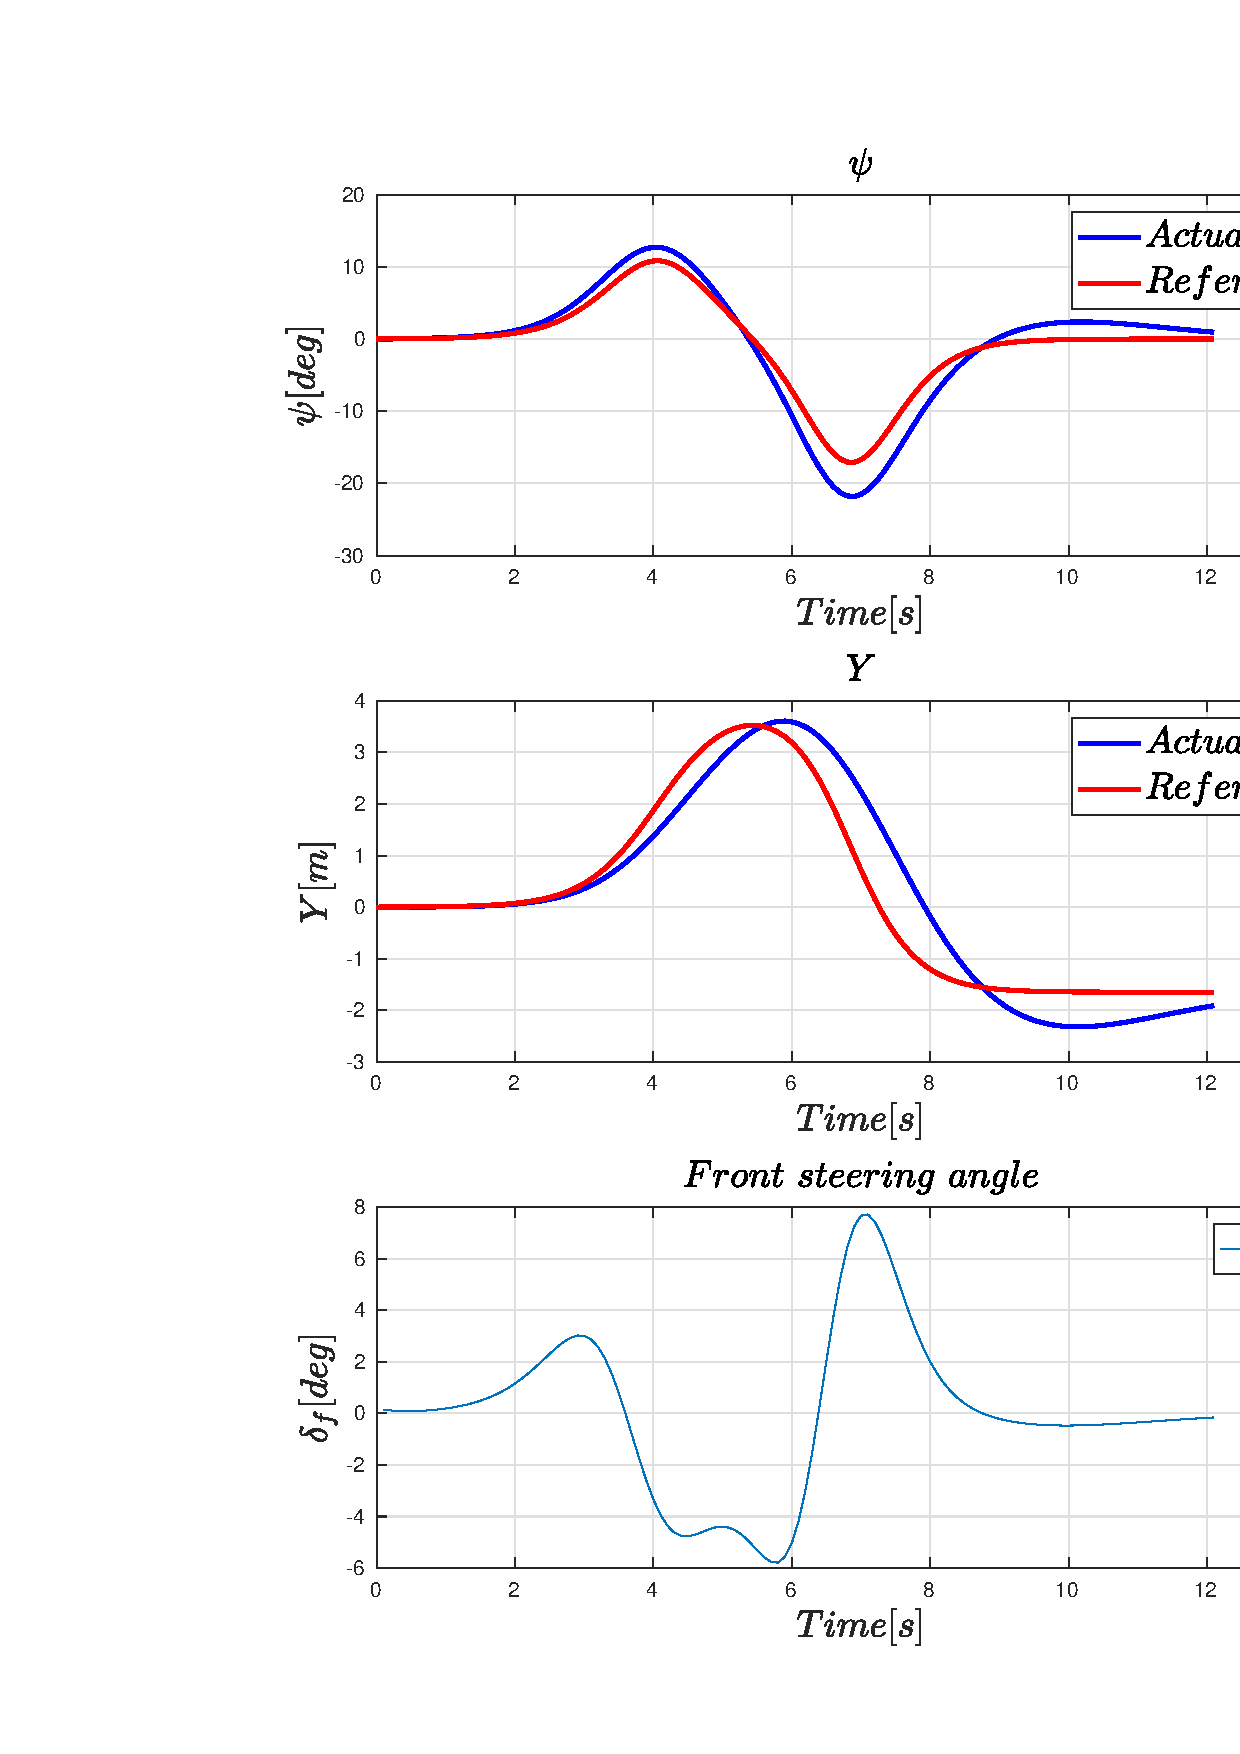
\includegraphics[width=0.95\textwidth,keepaspectratio]{images/Double_Lane_Change_Maneuver_MATLAB_01.pdf}
		\caption{(MATLAB) Double lane change maneuver at $10$ m/s with $H_p$ $=$ $7$ and $H_c$ $=$ $7$}
		\label{fig_07:double_lane_change_maneuver_01}
	\end{figure}
\end{frame}

\begin{frame}
	\frametitle{MATLAB Simulations via YALMIP Toolbox cont'd}
	\begin{figure}
		\centering
		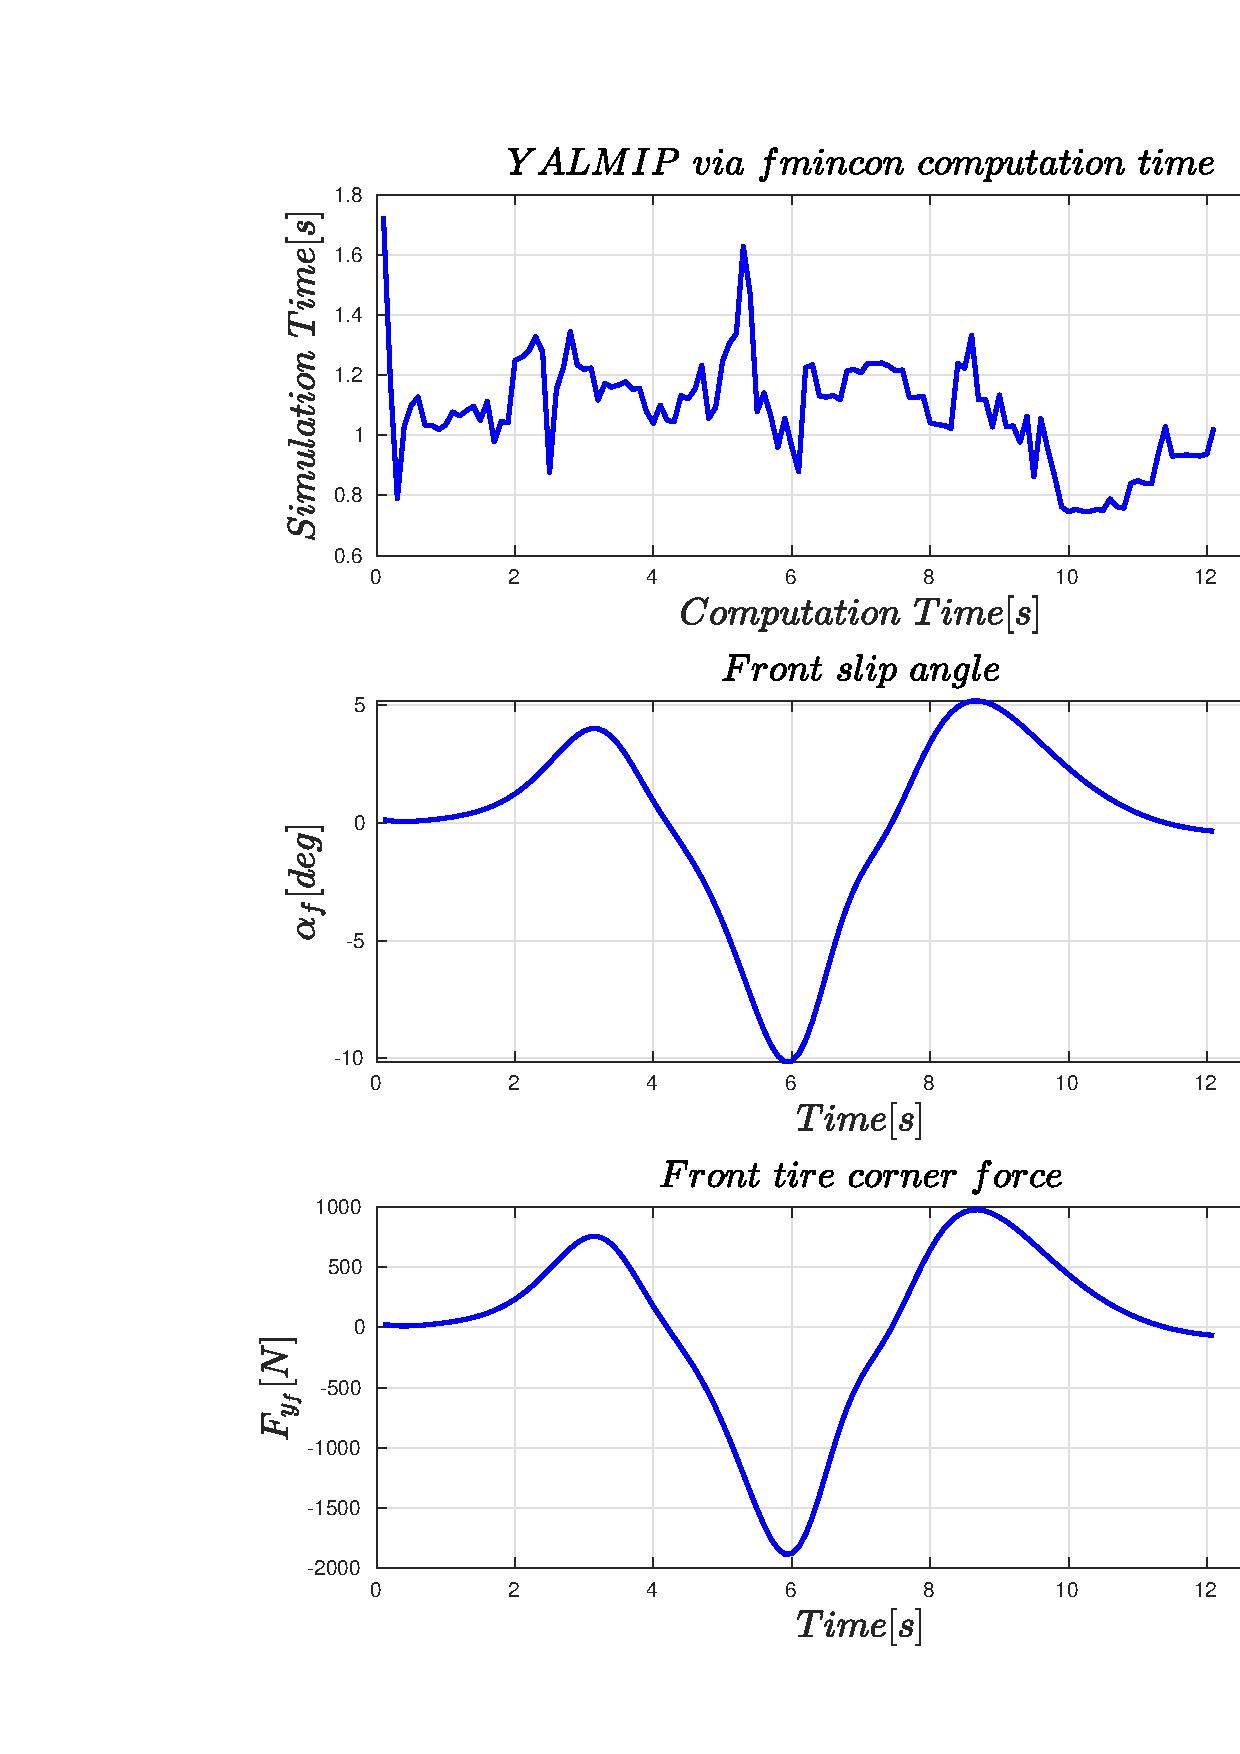
\includegraphics[width=0.95\textwidth,keepaspectratio]{images/Double_Lane_Change_Maneuver_MATLAB_02.pdf}
		\caption{(MATLAB) Double lane change maneuver at $10$ m/s with $H_p$ $=$ $7$ and $H_c$ $=$ $7$. YALMIP computation time, yaw rate, tire forces and slip angles.}
		\label{fig_08:double_lane_change_maneuver_02}
	\end{figure}
\end{frame}

\subsection{Simulation Results via C++ \& IPOPT, cppAD, matplotlibcpp}
\begin{frame}
	\frametitle{C++ Simulations via (IPOPT, cppAD, matplotlibcpp)}
	\begin{figure}
		\centering
		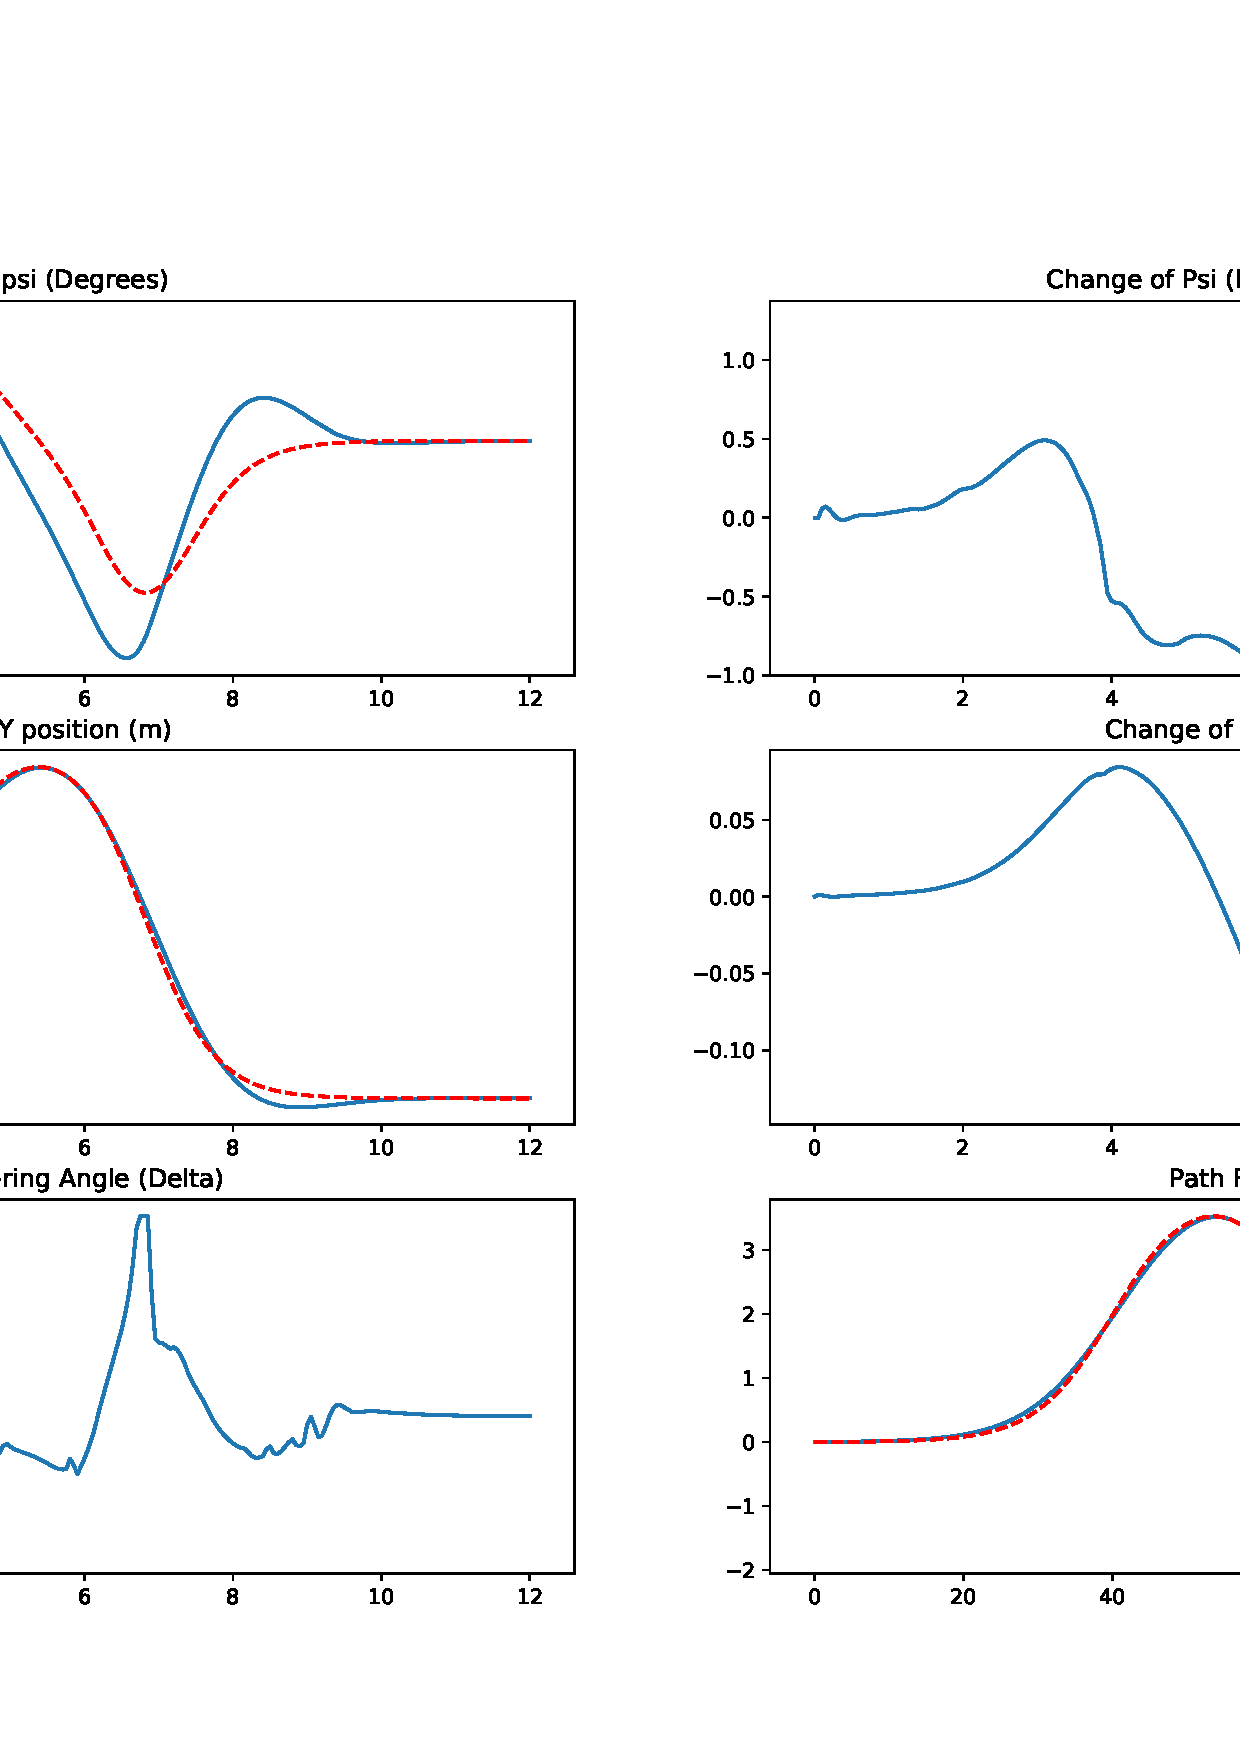
\includegraphics[width=0.95\textwidth,keepaspectratio]{images/Double_Lane_Change_Maneuver_cpp_01.pdf}
		\caption{(c++) Double lane change maneuver at $10$ m/s with $H_p$ $=$ $20$ and $H_c$ $=$ $20$}
		\label{fig_10:double_lane_change_maneuver_cpp_01}
	\end{figure}
\end{frame}

\begin{frame}
	\frametitle{C++ Simulations via (IPOPT, cppAD, matplotlibcpp) cont'd}
	\begin{figure}
		\centering
		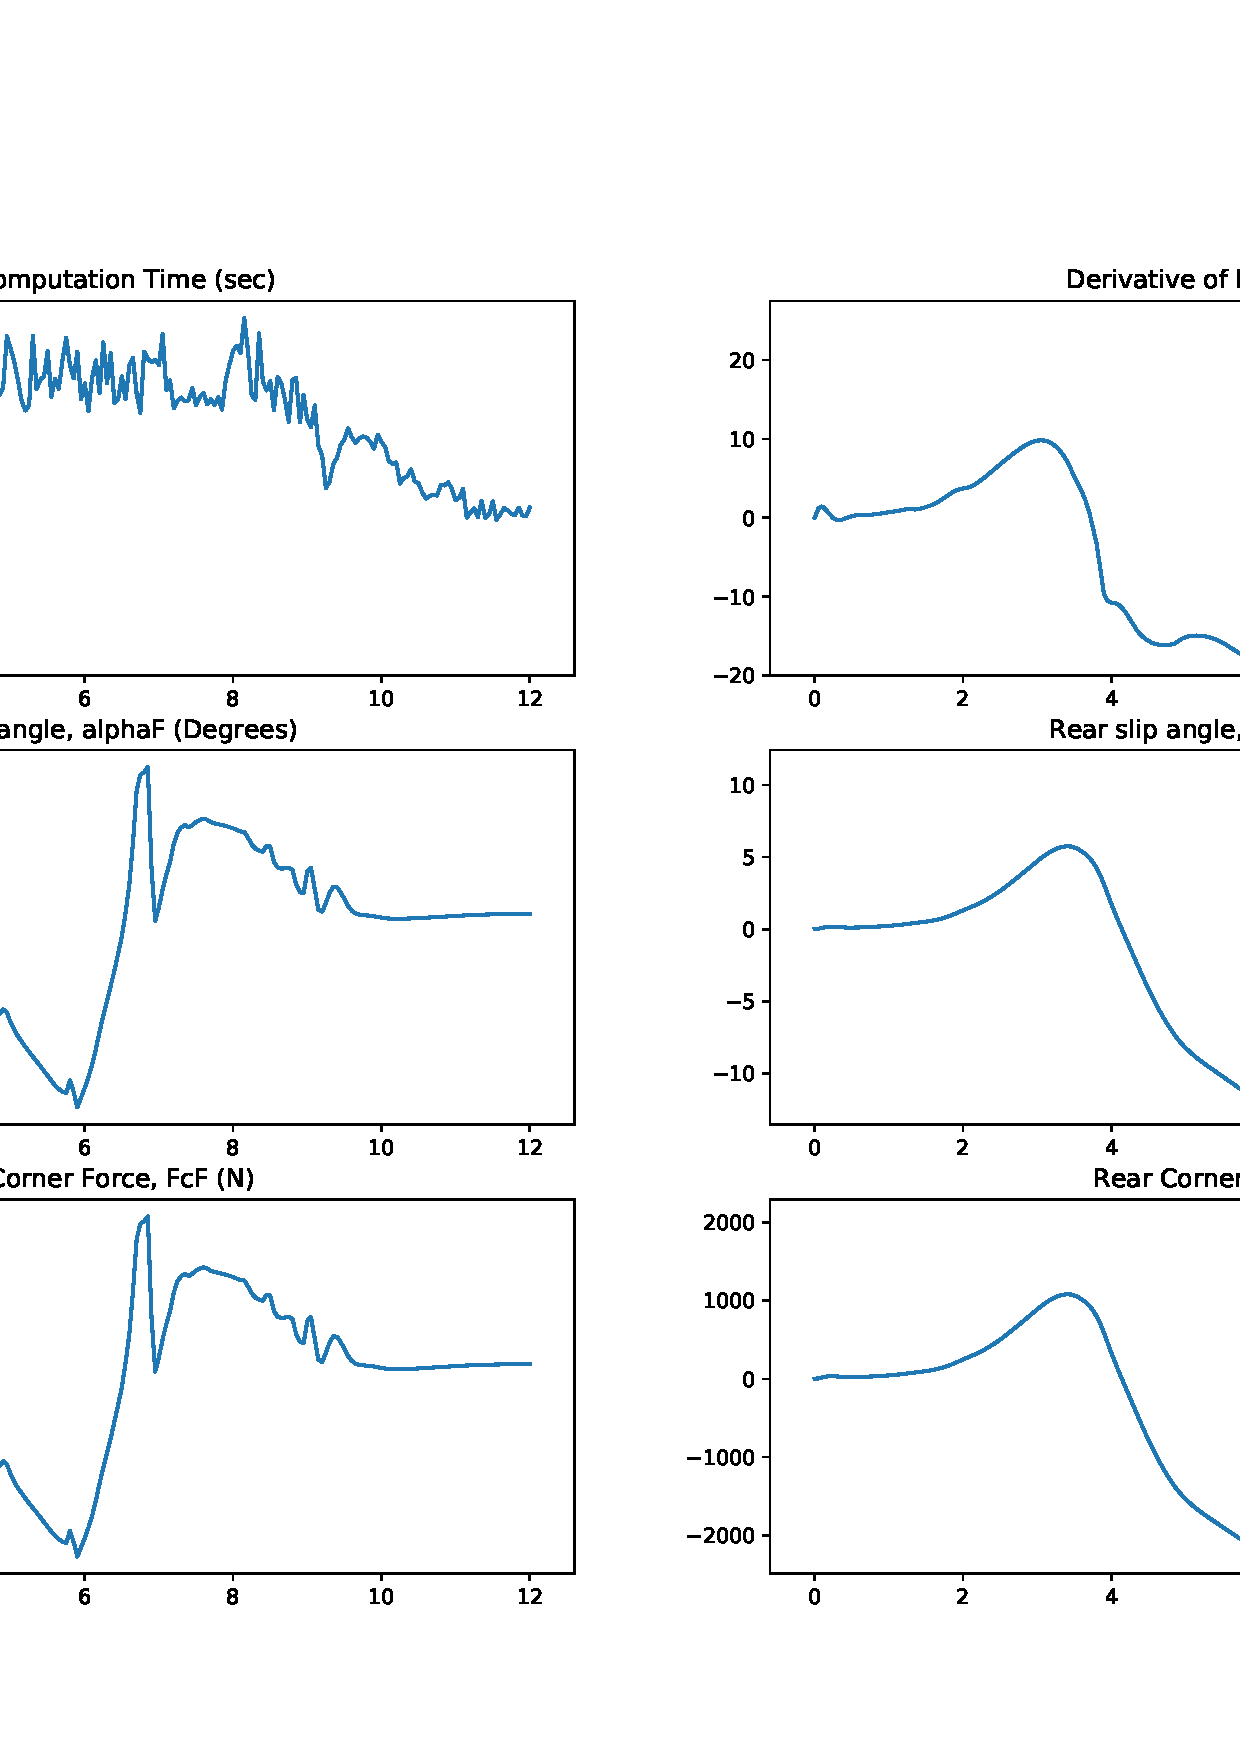
\includegraphics[width=0.95\textwidth,keepaspectratio]{images/Double_Lane_Change_Maneuver_cpp_02.pdf}
		\caption{(c++) Double lane change maneuver at $10$ m/s with $H_p$ $=$ $20$ and $H_c$ $=$ $20$. yaw rate, tire forces and slip angles.}
		\label{fig_11:double_lane_change_maneuver_02}
	\end{figure}
\end{frame}

\end{document}
